\section{Models}
\label{sec:models}

The sensor uses the photoelectric effect to produce output currents according to the following flow diagram:
\begin{figure}[H]
    \centering
    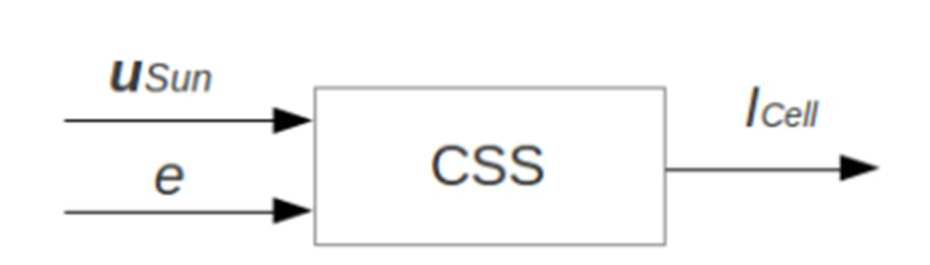
\includegraphics[width=0.5\linewidth]{doc//Graphics/sun_sensor_flowchart.png}
    \caption{Flow diagram for CSS}
    \label{fig:sun_sensor_model}
\end{figure}

The input Sun direction is given in the S/C frame. 
The CSS is also given the eclipse status of the 
S/C as a boolean $e$.
We need to take into account two configuration parameters: 1) the mounting orientation of the CSS with regard to the S/C and 2) the presence of a baffle, necessary to shield the sensor from stray light. 

\begin{figure}[H]
    \centering
    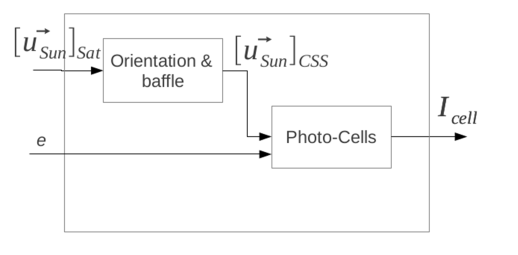
\includegraphics[width=0.75\linewidth]{Graphics/photo_cells_flowchart.png}
    \caption{Inner flow diagram for CSS}
    \label{fig:sun_sensor_inner_model}
\end{figure}

We decided to separate the model into the following submodels: \textit{Orientation and Baffle} and \textit{Cell}.
The Cell is implemented once for a single physical photo-cell and then combined in the CSS model with a total of four Cell models to accurately model the CSS.
Each submodel will be described further in the corresponding subsections below.

The configuration of the final CSS model can be seen below in \autoref{fig:CSS_model}.

\begin{figure}[H]
    \centering
    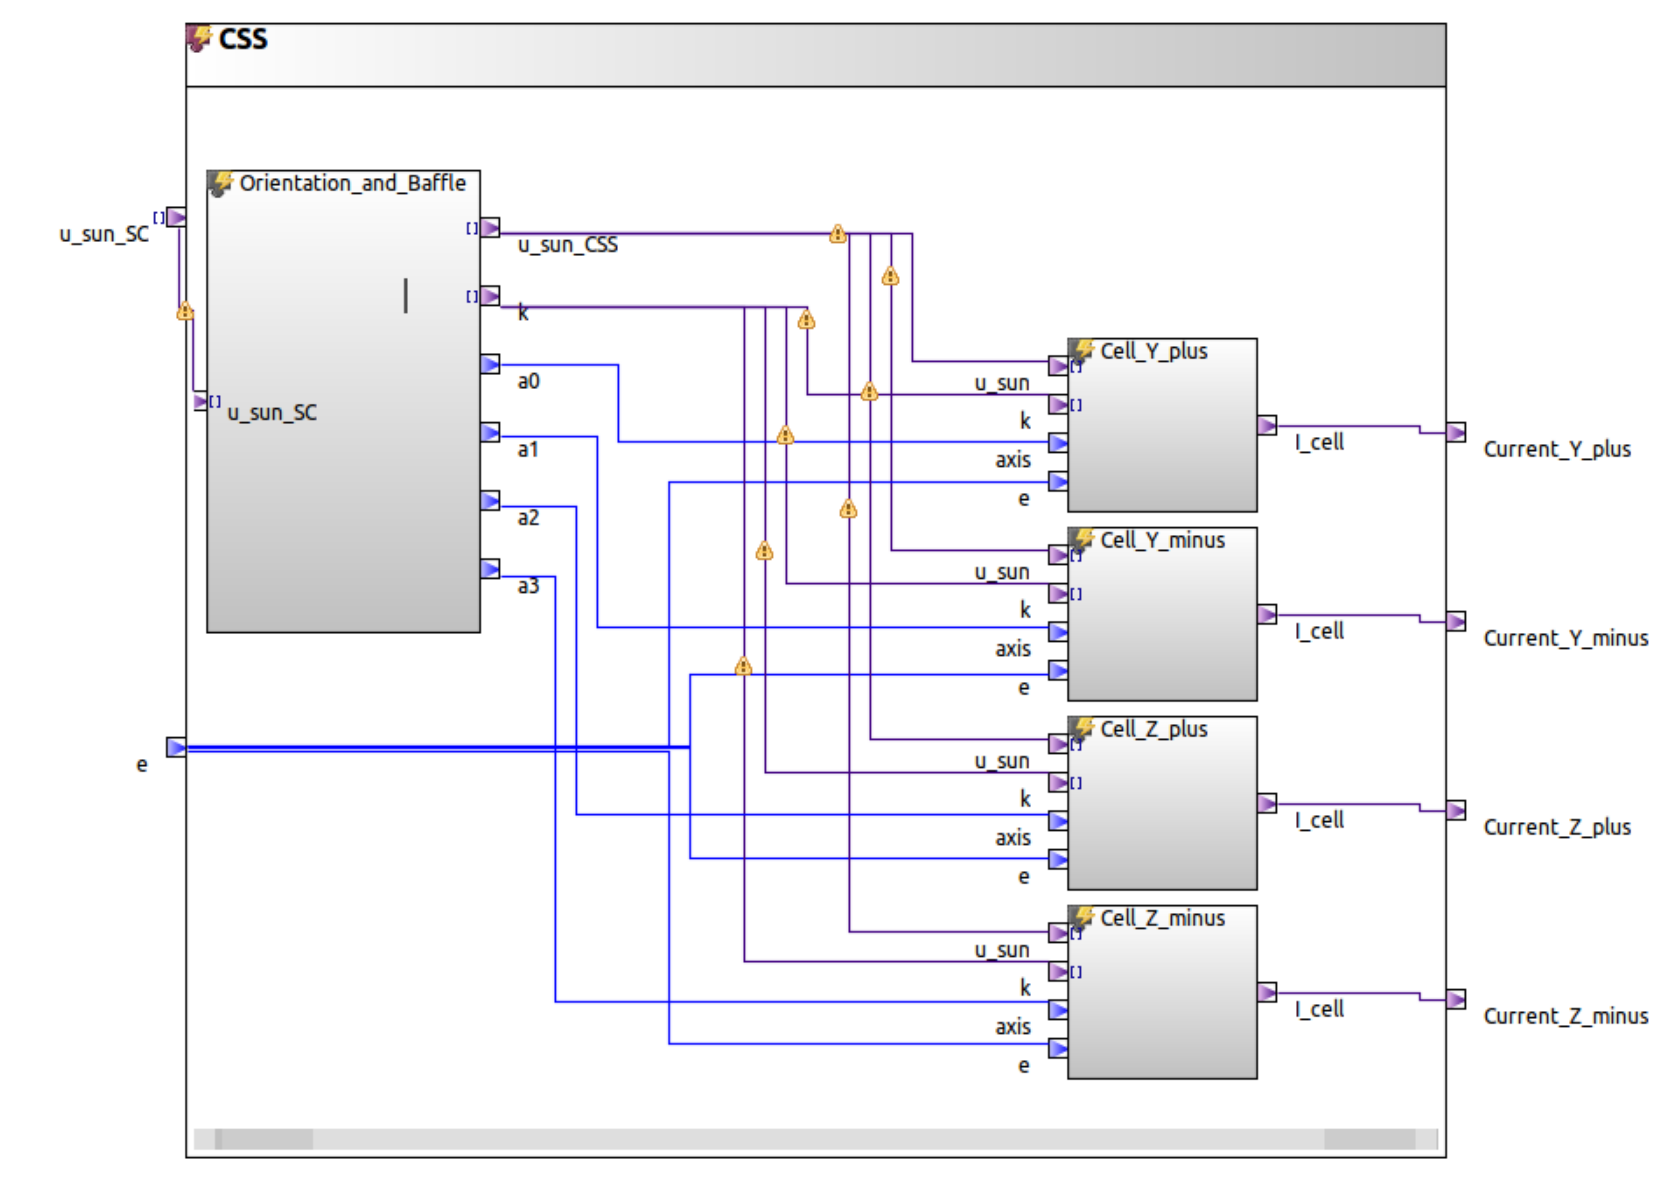
\includegraphics[width=1\linewidth]{doc//Graphics/CSS_model.png}
    \caption{SimTG model of CSS, \texttt{CSS.smf}}
    \label{fig:CSS_model}
\end{figure}



\subsection{Single Photo-Cell}

The output current from a single photo-cell does not have a linear response curve, especially when the incident light is away from the normal to the cell. 
The output current can be modelled with the following equation:
\begin{equation}
    \begin{split}
        &I_{cell} = I_{max} \times (\Vec{n} \cdot \Vec{u_{sun}} \times \lambda \times k \times e) + N(t) \\
        &\lambda = 1 - \left( \frac{2}{\pi} \times arccos(\Vec{n} \cdot \Vec{u_{sun}})\right)^v
    \end{split}
\end{equation}
where:
\begin{itemize}
    \item $I_{max}=31 \cdot 10^{-3} \, A$ is the maximal current the cell delivers for a Sun at the cell zenith
    \item $\Vec{n}$ is a unit vector normal to the cell
    \item $\Vec{u_{sun}}$ is the sun vector which contains the x-, y-, and z- values for the sun position given to the cell as input.
    \item $v = 9.6$ is the largest incident coefficient modelling the non-linearity of the cell
    \item $k \in [0,1]$ shows the influence of the baffle on the field-of-view limitation for each cell. $k=1$ when there is no obstacle between the Sun and the cell and $k=0$ when the Sun is completely hidden from the cell.
    \item $e$ is the eclipse status (0 if satellite is in Earth shadow). 
    \item $N(t)$ is a random white noise that will be added to the output. It is bound to the constant $N_{CSS} = 2.3 \cdot 10^{-10}\, A$ and its value varies randomly.
\end{itemize}

To model the single cell, we will need as inputs the sun vector ($\Vec{u_{sun}}$), the baffle coefficient ($k$) and the eclipse status ($e$).
It will also need as input which axis it is on since the full sun sensor consists of four solar cells. 
The solar cell then uses the axis value to deduce which normal vector ($\Vec{n}$) component it shall use for the calculations.
Note that the input $k$ is an array with 4 values, which is received from the \textit{Orientation and Baffle} model such that the indexes correspond to each specific cell (+Y, -Y, +Z and -Z).
In the model the correct k-value is then selected on based on which axis the specific cell is mounted on.

The cell produces the output of $I_{cell}$ based on these inputs, according to the SimTG model the \texttt{Cell.smf}-file which is shown below in \autoref{fig:cell_model}.

\begin{figure}[H]
    \centering
    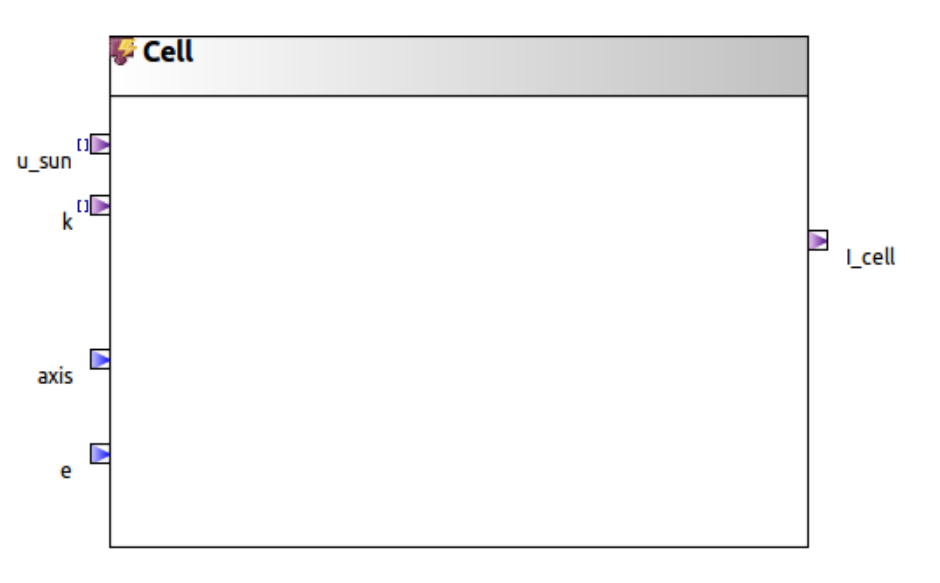
\includegraphics[width=0.7\linewidth]{doc//Graphics/cell_model.png}
    \caption{SimTG model of single photo cell, \texttt{Cell.smf}.}
    \label{fig:cell_model}
\end{figure}

The calculation of the output current for a single photo-cell is done in a \texttt{Cell.cpp} cell, where the most relevant section is the \texttt{Cell::step()} method, which can be seen below:
\begin{lstlisting}[frame=single, numbers=left, basicstyle=\tiny, language = C++]
void Cell::step() throw (simtg::Exception) {
	/*PROTECTED REGION ID(_bDafA9NTEe-HHfwhf86eRQ) ENABLED START*/
	float alpha = 22 * (M_PI / 180);		// sunsensor angle, converted to rad
	float I_max = 31.0 / 1000;			// max current in [A]
	float v = 9.6;						// largest incident coeff [-]
	//float N_CSS = 2.3 * pow(10, -10);	// Noise coefficient
	//float N = static_cast<float>(rand()) / (static_cast<float>(RAND_MAX / N_CSS)); // Noise
	float N = 0.0;

	float n[4][3];
	n[0][0] = sin(alpha);
	n[0][1] = cos(alpha);
	n[0][2] = 0;
	n[1][0] = sin(alpha);
	n[1][1] = -cos(alpha);
	n[1][2] = 0;
	n[2][0] = sin(alpha);
	n[2][1] = 0;
	n[2][2] = cos(alpha);
	n[3][0] = sin(alpha);
	n[3][1] = 0;
	n[3][2] = -cos(alpha);

	float dotProd = (_u_sun[0] * n[_axis][0]) + (_u_sun[1] * n[_axis][1])
			+ (_u_sun[2] * n[_axis][2]);

	float lambda = 1 - pow(((2 / M_PI) * acos(dotProd)), v);

	_I_cell = ((I_max * (dotProd * lambda * _k[_axis] * _e)) + N);
	/*PROTECTED REGION END*/
}
\end{lstlisting}








\subsection{Orientation and Baffle}
The sun sensor is nominally mounted in such a way that $X_C$ is along the $-Z_S$-axis, $Y_C$ is along the $+Y_S$-axis and $Z_C$ is along the $+X_S$-axis. 
We must therefore use a rotation matrix to go from the S/C frame to the sun-sensor frame.
The used rotation matrix is:

\begin{equation}
M_R = 
\begin{bmatrix}
    cos(90^\circ) & 0 & sin(90^\circ)\\
    0 & 1 & 0 \\
    -sin(90^\circ) & 0 & cos(90^\circ)
\end{bmatrix}	
\end{equation}

This translates in the end to an operation where the original $\Vec{u}_{sun}$ is simply reversed, as can be seen in the code below:
\begin{lstlisting}[frame=single, numbers=left, basicstyle=\tiny, language=c++]
// Convert reference frame
_u_sun_CSS[0] = -_u_sun_SC[2];
_u_sun_CSS[1] = _u_sun_SC[1];
_u_sun_CSS[2] = _u_sun_SC[0];
\end{lstlisting}

\vspace{0.5cm}

Within the Orientation and Baffle model we also define the axis outputs, which will be the inputs for each single photo cell. In other words, we model four cells so we give out four axis outputs which each go into one of the four cells. The values of these axis outputs are [0, 1, 2, 3] and the single cell knows then which $\Vec{n}$ component to used based on the axis input.


The sensor is equipped with a mission-specific baffle to avoid reflections from S/C parts having a negative effect on the measurement accuracy. 
The baffle takes into account the physical limitation in the CSS field-of-view. 
It is modeled as a black wall surrounding the CSS in order to protect it from stray light and is visualised in the left image in \autoref{fig:baffle_theory}.
The wall is placed at a definite distance from the cell, blinding it when the Sun goes below the wall horizon. The effect of the baffle on the output current can be approximated by a coefficient $k$ as follows:
\begin{itemize}
    \item $\theta < \theta_{\min} \Rightarrow k = 1$
    \item $\theta_{\min} \leq \theta \leq \theta_{\max} \Rightarrow k = \frac{\sin(\theta_{\max} - \theta)}{\sin(\theta_{\max} - \theta_{\min})}$
    \item $\theta > \theta_{\max} \Rightarrow k = 0$
\end{itemize}

\vspace{0.5cm}
The values of the limit co-elevation angles depend on the baffle geometry and are functions of the Sun azimuth in the CSS frame. 
Moreover, these angles are relative to the considered cell. The precise calculation of the limit angles extracted from a particular geometry being a tedious task, the baffle is approximated by a set of 40 azimuthal sectors of 9 degrees centred on the CSS axis and the bisecting lines of the Yc and Zc axis, which is visualised in the right image in \autoref{fig:baffle_theory}.
Note that the first sector begin at Azimuth 355.5° and end at Azimuth 4.5°. 
The cells are numbered counter-clockwise. 
The values of the limit angles by sector by cells and some diagrams are given in the exercise sheet appendix.



\begin{figure}[H]
    \centering
    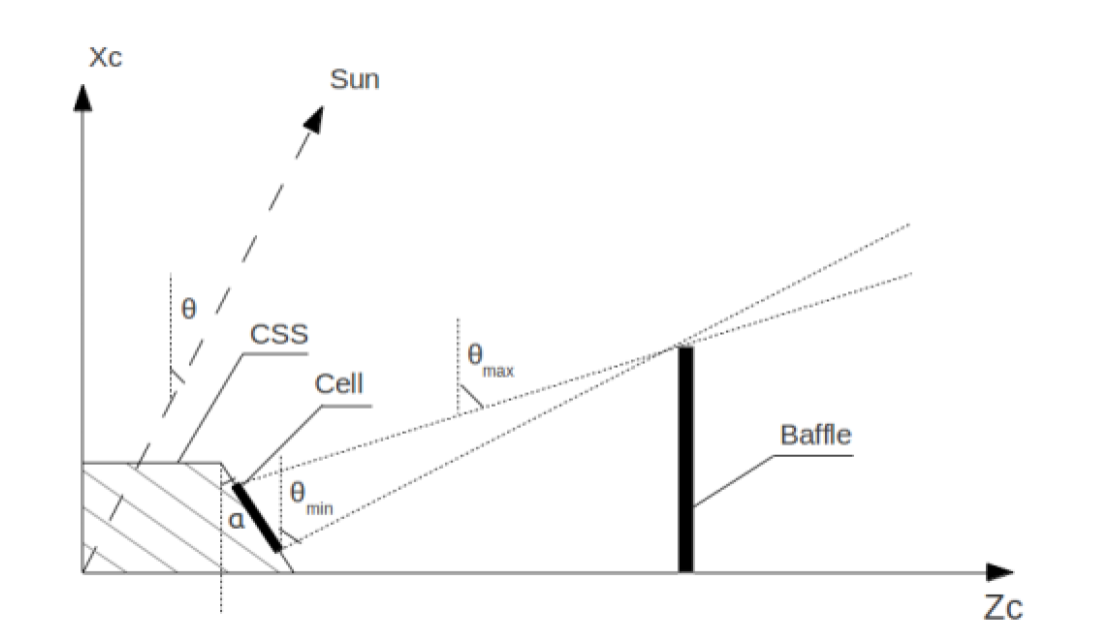
\includegraphics[width=0.45\linewidth]{doc//Graphics/baffle_geometry.png}
    \hfill
    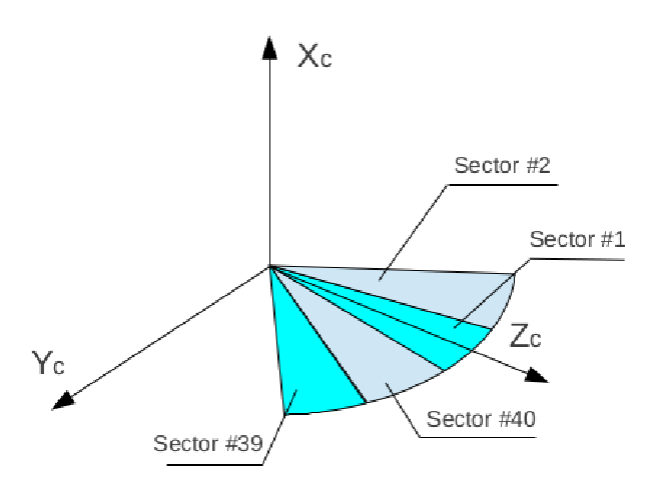
\includegraphics[width=0.45\linewidth]{doc//Graphics/baffle_sectors.png}
    \caption{Baffle geometry and sector definition}
    \label{fig:baffle_theory}
\end{figure}


In modelling the baffle, we first take the values from the Baffle definition in the exercise sheet and define them as static arrays in the Orientation and Baffle model .cpp code. This is done at the beginning of the file so that we don't have to consider keeping them in a .csv file and doing file operations, but instead, they can be called at any time based on which sector we are in. This sector then corresponds to the index of each static array, such that each column in the exercise sheet is one separate static array. We can then utilise a for loop to loop through each of these values when calculating the baffle and finally setting the separate $k$-values for each individual cell in our four-cell configuration. The cells then know themselves which axis they are on and can use the correct corresponding $k$-value. We use the following for-loop (which is also defined in the beginning of the \texttt{Orientation\_and\_baffle.cpp} file) to get the k-value:
\begin{lstlisting}[frame=single, numbers=left, basicstyle=\tiny, language=c++]
float get_k(float elev, float theta_min, float theta_max) {
    elev = elev * M_PI/180.0;
    theta_min = theta_min * M_PI / 180.0;
    theta_max = theta_max * M_PI / 180.0;
    
    if (elev < theta_min) {return 1.0;}
    else if (elev >= theta_min && elev <= theta_max) {return (sin(theta_max-theta_min));}
    else if (elev > theta_max) {return 0.0;}
    else {return 0.0;}
 }
\end{lstlisting}




The SimTG model of the Orientation and Baffle can be seen below in \autoref{fig:ori_model}.


\begin{figure}[H]
    \centering
    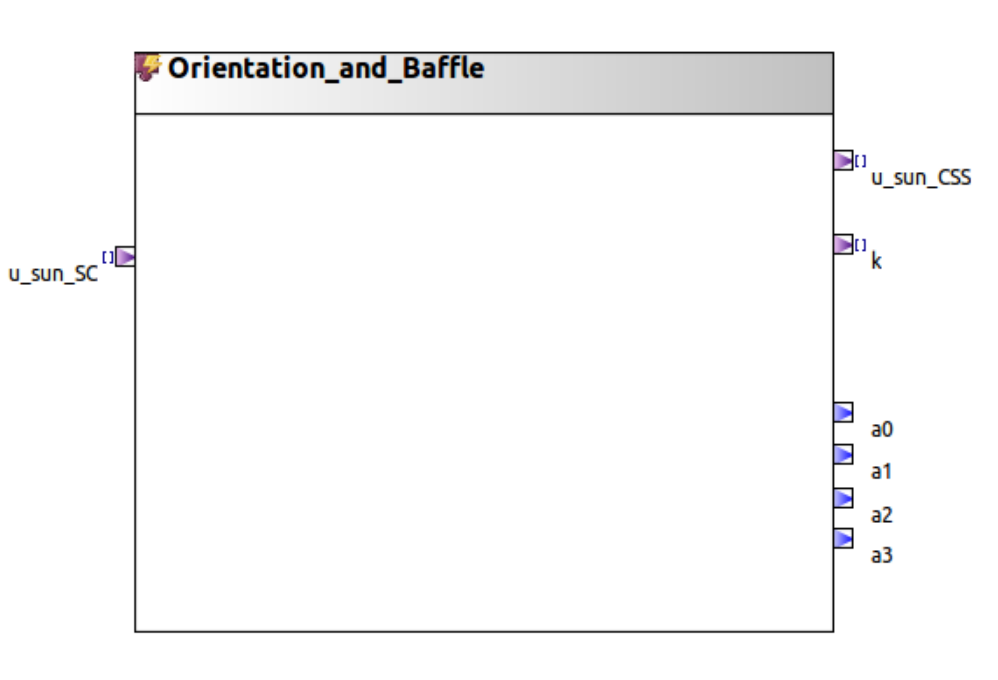
\includegraphics[width=0.6\linewidth]{doc//Graphics/ori_model.png}
    \caption{SimTG model of Orientation and Baffle, \texttt{Orientation\_and\_Baffle.smf}}
    \label{fig:ori_model}
\end{figure}



\newpage
\subsection{Controller}
%\TODO{Henkka lisää tekstiä control hommelista + see hieno lohkokaavio!}
\begin{figure}[H]
    \centering
    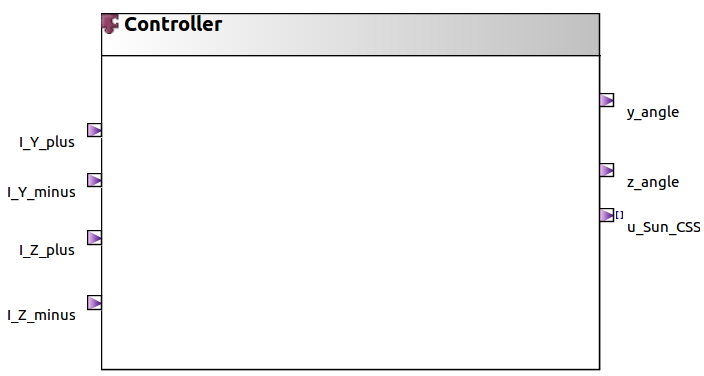
\includegraphics[width=0.6\linewidth]{doc//Graphics/controllerModel.png}
    \caption{The controller model.}
    \label{fig:controllerModel}
\end{figure}

The controller takes the electric current of each CSS as an input, and outputs the new Sun vector in CSS coordinates. It works by taking the difference between the opposite sun sensors and feeding that into a PID. The reference signal is set to 0 because the sun sensors are facing towards the Sun when there is no difference between the currents, i.e. the angles between the sun sensors and the Sun are equal. After that, the angle is used to calculate a new direction for the Sun, which is fed back to the sun sensors, completing the feedback loop. The output from y-axis PID controls the actuator for z-axis, and the output from z-axis PID controls the actuator for y-axis.

\subsection{Satellite}
\begin{figure}[H]
    \centering
    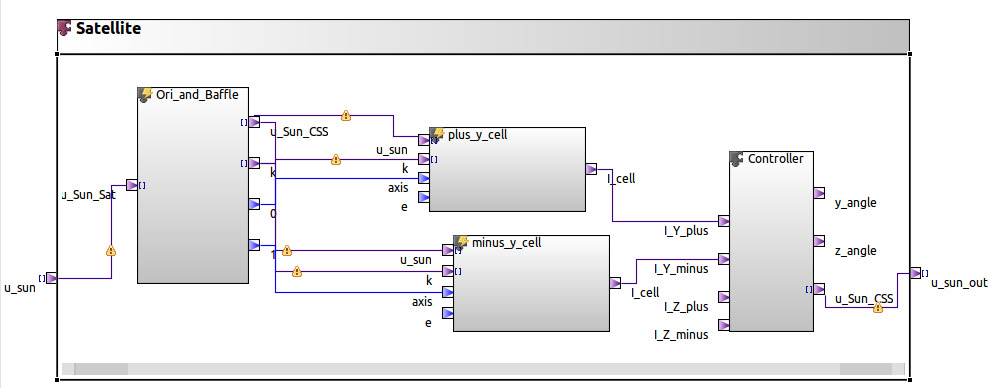
\includegraphics[width=1.0\linewidth]{doc//Graphics/satellite.png}
    \caption{The satellite model for testing}
    \label{fig:satelliteModel}
\end{figure}

Satellite is the final model to encompass the whole system inside of it. It takes the Sun's direction as an input in satellite coordinates, transforms it into the CSS coordinates, generates the electric current for +Y and -Y sun sensors, and finally the controller calculates the new Sun direction, which is the output. 

The model which is used here is not complete, because it is not using the actual CSS model. Therefore, it is missing the z-axis cells. This model is used for testing because of its simplicity, and easier access to read the sub-model values. The design for the complete satellite can be seen below.

\begin{figure}[H]
    \centering
    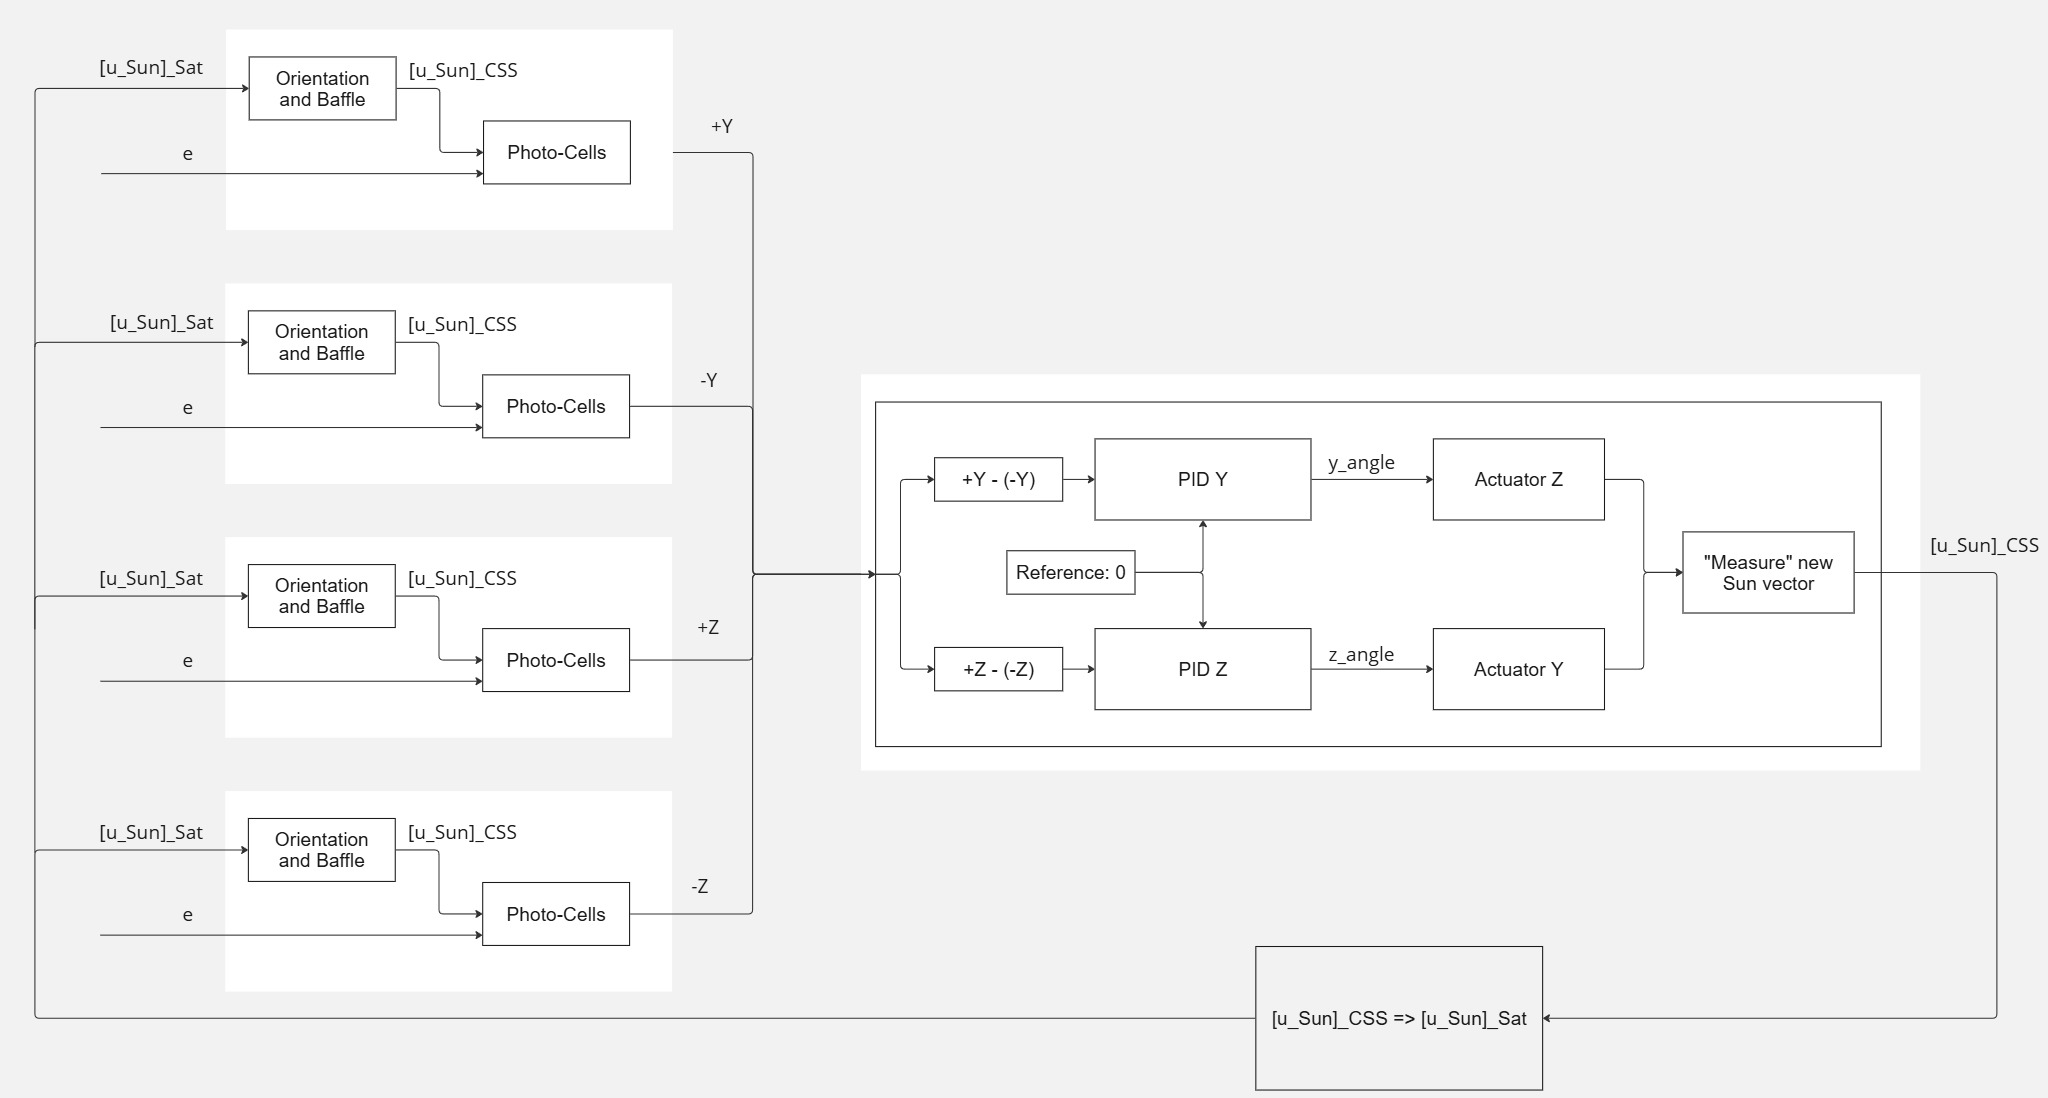
\includegraphics[width=1.0\linewidth]{doc//Graphics/controller.jpg}
    \caption{Design of the satellite.}
    \label{fig:satelliteDesign}
\end{figure}
